 \section{Expansi'on hasta orden cuadr'atico en \texorpdfstring{$G$}{G}}
\subsubsection{M'etrica}

Ahora obtendremos una expresi'on para las ecuaciones de Einstein a segundo orden, es decir, aquellas que son cuadr'aticas en la constante gravitacional. Naturalmente, esta ecuaci'on de segundo orden en nuestro esquema perturbativo depender'a linealmente de la perturbaci'on de segundo orden de la m'etrica $h^{(2)}_{\mu\nu}$ y cuadr'aticamente de la perturbaci'on de primer orden $h^{(1)}_{\mu\nu}$.

Calculamos primero la perturbaci'on de orden 2 de la m'etrica inversa, que resulta ser 
\begin{equation}
g^{\mu\nu}_{(2)}=-h^{\mu\nu}_{(2)}+ h^{\mu\lambda}_{(1)}h_{(1)}{}_\lambda^{\ \nu} ,
\end{equation}
y donde hemos usado una notaci'on similar a la usada para las perturbaciones de primer orden para simbolizar las contracciones con la m'etrica plana $\eta$.

\subsubsection{Conexi'on}
Similarmente, la perturbaci'on de orden 2 de la conexi'on tiene la forma
\begin{equation}
\Gamma^\lambda_{(2)\mu\nu}=\frac{1}{2}\left(\partial_\mu h^\lambda_{(2)\nu} + \partial_\nu h^\lambda_{(2)\mu} -\partial^\lambda h^{(2)}_{\mu\nu}\right)
-\frac{1}{2}h_{(1)}^{\lambda\rho}\left(\partial_\mu
h^{(1)}_{\nu\rho} +\partial_\nu h^{(1)}_{\mu\rho} - \partial_\rho h^{(1)}_{\mu\nu}\right).
\end{equation}

\subsubsection{Tensor de Ricci}
Por otro lado, la componente cuadr'atica en $G$ del tensor de Ricci puede escribirse como
\begin{align}
R^{(2)}_{\mu\lambda} = &\ \frac{1}{2}\left(\partial_\mu\partial_\nu h^\nu_{(2)\lambda}+ \partial_\lambda \partial^\nu h^{(2)}_{\mu\nu} - \partial_\mu\partial_\lambda h^{(2)} -\square h^{(2)}_{\mu\lambda}\right) \\
& +\frac{1}{2}\left[\frac{1}{2}(\partial_\lambda h^{\sigma\rho}_{(1)})(\partial_\mu h_{\sigma\rho}^{(1)})+h^{\sigma\rho}_{(1)}\left(\partial_\lambda\partial_\mu h^{(1)}_{\sigma\rho}-\partial_\rho\partial_\mu h^{(1)}_{\lambda\sigma}-\partial_\rho\partial_\lambda h^{(1)}_{\mu\sigma}+ \partial_\rho\partial_\sigma h^{(1)}_{\mu\lambda}\right) \right.\\
& \left.+ (\partial_\sigma h^\rho_{(1)\lambda})\left(\partial^\sigma h^{(1)}_{\mu\rho}-\partial_\rho h^\sigma_{(1)\mu}\right) -\partial_\rho\left(h^{\sigma\rho}_{(1)}-\frac{1}{2}\eta^{\sigma\rho}\,h^{(1)}\right)\left(\partial_\mu h^{(1)}_{\lambda\sigma}+\partial_\lambda h^{(1)}_{\mu\sigma}-\partial_\sigma h^{(1)}_{\mu\lambda}\right) \right]\\
=&\ \frac{1}{2}\left(\partial_\mu\partial_\nu h^\nu_{(2)\lambda}+ \partial_\lambda \partial^\nu h^{(2)}_{\mu\nu} - \partial_\mu\partial_\lambda h^{(2)} -\square h^{(2)}_{\mu\lambda}\right) +A_{\mu\lambda},
\end{align}
donde hemos definido
\begin{align}
A_{\mu\lambda} := & \ \frac{1}{2}\left[\frac{1}{2}(\partial_\lambda h^{\sigma\rho}_{(1)})
(\partial_\mu h_{\sigma\rho}^{(1)})+h^{\sigma\rho}_{(1)}
\left(\partial_\lambda\partial_\mu h^{(1)}_{\sigma\rho}-\partial_\rho\partial_\mu
h^{(1)}_{\lambda\sigma}-\partial_\rho\partial_\lambda h^{(1)}_{\mu\sigma}
+ \partial_\rho\partial_\sigma h^{(1)}_{\mu\lambda}\right) \right. \nonumber\\
& + \left.  (\partial_\sigma h^\rho_{(1)\lambda})\left(\partial^\sigma h^{(1)}_{\mu\rho}-\partial_\rho h^\sigma_{(1)\mu}\right) -\partial_\rho\left(h^{\sigma\rho}_{(1)}-\frac{1}{2}\eta^{\sigma\rho}\,h^{(1)}\right)\left(\partial_\mu h^{(1)}_{\lambda\sigma}+\partial_\lambda h^{(1)}_{\mu\sigma}-\partial_\sigma h^{(1)}_{\mu\lambda}\right) \right]. \label{defAmn}
\end{align}

\subsubsection{Escalar de Curvatura}
La correspondiente componente del escalar de curvatura resulta ser
\begin{align}
R^{(2)} = &\ \eta^{\mu\nu}R^{(2)}_{\mu\nu}-h_{(1)}^{\mu\nu}R^{(1)}_{\mu\nu} \\
= &\ \partial^\mu\partial^\nu h^{(2)}_{\mu\nu} - \square h^{(2)}
-\frac{1}{2}h_{(1)}^{\mu\lambda}\left(2\partial_\mu\partial_\nu h^\nu_{(1)\lambda}
- \partial_\mu\partial_\lambda h^{(1)} -\square h^{(1)}_{\mu\lambda}\right)
+ \eta^{\mu\nu}A_{\mu\nu} \\
= &\ \partial^\mu\partial^\nu h^{(2)}_{\mu\nu} - \square h^{(2)}
+h_{(1)}^{\sigma\rho}\left(\square h^{(1)}_{\sigma\rho}
-2\partial_\rho\partial_\nu \bar{h}^\nu_{(1)\sigma}\right)
+\frac{3}{4}(\partial^\mu h_{(1)}^{\sigma\rho})(\partial_\mu h^{(1)}_{\sigma\rho}) \\
& -\frac{1}{2}(\partial^\sigma h_{(1)}^{\rho\mu})(\partial_\rho h^{(1)}_{\sigma\mu})
-(\partial_\rho h_{(1)}^{\sigma\rho})(\partial_\mu \bar{h}^\mu_{(1)\sigma})
+\frac{1}{2}(\partial^\nu h^{(1)})(\partial_\mu \bar{h}^\mu_{(1)\nu})\\
= &\ \partial^\mu\partial^\nu h^{(2)}_{\mu\nu} - \square h^{(2)}
+B,
\end{align}
con
\begin{align}
B := &\ h_{(1)}^{\sigma\rho}\left(\square h^{(1)}_{\sigma\rho}
-2\partial_\rho\partial_\nu \bar{h}^\nu_{(1)\sigma}\right)
+\frac{3}{4}(\partial^\mu h_{(1)}^{\sigma\rho})(\partial_\mu h^{(1)}_{\sigma\rho}) -\frac{1}{2}(\partial^\sigma h_{(1)}^{\rho\mu})(\partial_\rho h^{(1)}_{\sigma\mu}) \nonumber \\
& -(\partial_\rho h_{(1)}^{\sigma\rho})(\partial_\mu \bar{h}^\mu_{(1)\sigma})
+\frac{1}{2}(\partial^\nu h^{(1)})(\partial_\mu \bar{h}^\mu_{(1)\nu})
. \label{defB}
\end{align}

\subsubsection{Tensor de Einstein}
Finalmente, la contribuci'on cuadratica en $G$ al tensor de Einstein es dada por
\begin{align}
G^{(2)}_{\mu\nu} & =  R^{(2)}_{\mu\nu}-\frac{1}{2}\eta_{\mu\nu}R^{(2)}-\frac{1}{2}h^{(1)}_{\mu\nu}R^{(1)}\\
& =  \frac{1}{2}\left[\partial_\mu\partial^\lambda h^{(2)}_{\lambda\nu}
+\partial_\nu\partial^\lambda h^{(2)}_{\lambda\mu} -
\partial_\mu\partial_\nu h^{(2)} -\square h^{(2)}_{\mu\nu}
-\eta_{\mu\nu}\left(\partial^\lambda \partial^\rho h^{(2)}_{\lambda\rho}
- \square h^{(2)}\right) \right]+C_{\mu\nu},
\end{align}
con
\begin{align}
C_{\mu\lambda} :=&\  A_{\mu\lambda}-\frac{1}{2}\,\eta_{\mu\lambda}\, B-\frac{1}{2}h^{(1)}_{\mu\lambda}R^{(1)}.
\end{align}
En t'erminos de $\bar{h}^{(2)}_{\mu\nu}$, tenemos
\begin{align}
G^{(2)}_{\mu\nu} = & -\frac{1}{2}\left[\square \bar{h}^{(2)}_{\mu\nu}
+\eta_{\mu\nu}\, \partial^\lambda\partial^\rho\bar{h}^{(2)}_{\lambda\rho}-
\partial_\mu\partial^\lambda\bar{h}^{(2)}_{\lambda\nu}
- \partial_\nu\partial^\lambda \bar{h}^{(2)}_{\lambda\mu}\right]
+C_{\mu\nu}.
\end{align}

Note que las todas las expresiones para las perturbaciones de segundo orden dependen de la perturbaci'on $h^{(2)}_{\mu\nu}$ exactamente de la misma forma que las expresiones de primer orden dependen de $h^{(1)}_{\mu\nu}$. Esto es consecuencia de la expansi'on de estamos realizando (en torno a la m'etrica plana, de orden 0), y de la consistencia de la separaci'on realizada de las ecuaciones de Einstein en t'erminos que dependen de distintas potencias de $G$. Como vemos, lo que diferencia las expresiones de segundo orden es que adem'as poseen t'erminos, necesariamente sumados a los primeros, que dependen cuadr'aticamente de (las derivadas de) $h^{(1)}_{\mu\nu}$.


\section{Ecuaciones de Einstein a segundo orden}
De esta forma, las ecuaciones de Einstein de segundo orden son
\begin{equation}\label{lee2g2}
\square \bar{h}^{(2)}_{\mu\nu}
+\eta_{\mu\nu}\, \partial^\lambda\partial^\rho\bar{h}^{(2)}_{\lambda\rho}-
\partial_\mu\partial^\lambda\bar{h}^{(2)}_{\lambda\nu}
- \partial_\nu\partial^\lambda \bar{h}^{(2)}_{\lambda\mu} -2C_{\mu\nu}=
-\frac{16\pi G}{c^4}T_{\mu\nu}^{(1)} \, ,
\end{equation}
o, llevando el t'ermino $C_{\mu\nu}$ al lado derecho,
\begin{equation}\label{lee2g3}
\boxed{\square \bar{h}^{(2)}_{\mu\nu}
+\eta_{\mu\nu}\, \partial^\lambda\partial^\rho\bar{h}^{(2)}_{\lambda\rho}-
\partial_\mu\partial^\lambda\bar{h}^{(2)}_{\lambda\nu}
- \partial_\nu\partial^\lambda \bar{h}^{(2)}_{\lambda\mu} =
-\frac{16\pi G}{c^4}\left(T_{\mu\nu}^{(1)}+t_{\mu\nu} \right)\, .}
\end{equation}
Aqu'i hemos introducido
\begin{equation}
t_{\mu\nu}:=-\frac{c^4}{8\pi G}\,C_{\mu\nu}, \label{deft}
\end{equation}
que se suma a la contribuci'on de primer orden del tensor de energ'ia-momentum de la materia. El lado derecho de (\ref{lee2g3}) depende de la distribuci'on de materia (que se supone conocida) y de $h^{(1)}_{\mu\nu}$. De esta forma, (\ref{lee2g3}) suministra una ecuaci'on para la perturbaci'on de segundo orden $h^{(2)}_{\mu\nu}$, que tiene la misma forma que aquella para la perturbaci'on de primer orden, ec. (\ref{lee}), pero con un ``t'ermino fuente'' dependiente de la distribuci'on de materia y de la perturbaci'on de primer orden de la m'etrica. Adem'as, tal como en el caso de primer orden, la cuadridivergencia del lado izquierdo de (\ref{lee2g3}) es id'enticamente nula por lo que, como consecuencia,
\begin{equation}
\partial_\nu\left(T^{\mu\nu}_{(1)}+t^{\mu\nu} \right)=0. \label{cTt}
\end{equation}
En otras palabras, y esta vez a diferencia de lo encontrado a primer orden, la correspondiente componente del tensor de energ'ia-momentum de la materia \textit{no es conservado por separado}, sino s'olo su suma con el (pseudo-)tensor (\ref{deft}). Puesto que $t^{\mu\nu}$ depende (cuadr'aticamente) de $h^{(1)}_{\mu\nu}$, es posible interpretarlo como un \textbf{tensor de energ'ia-momentum efectivo para campo gravitacional}. Entonces (\ref{cTt}) representa la conservaci'on, correcta hasta el orden lineal en $G$, de la energ'ia y el momentum total del sistema materia + campo gravitacional. Equivalentemente, sumando (\ref{cTt}) y (\ref{cT0}) podemos escribir
\begin{equation}
\boxed{\partial_\nu\left(T^{\mu\nu}_{(0,1)}+t^{\mu\nu} \right)=0,} \label{cT01t}
\end{equation}
donde $T^{\mu\nu}_{(0,1)}:=T^{\mu\nu}_{(0)}+T^{\mu\nu}_{(1)}$ es el tensor de energ'ia-momentum de las fuentes, correcto hasta orden lineal en $G$.

\subsection{Gauges}
A segundo orden,
\begin{align}\label{pc2}
h'^{(2)}_{\mu\nu} = &\ h^{(2)}_{\mu\nu}- \partial_\mu\xi_\nu^{(2)} - \partial_\nu\xi_\mu^{(2)}\\
&  -(\partial_\nu\xi^\rho_{(1)})h^{(1)}_{\mu\rho} -(\partial_\mu\xi^\lambda_{(1)})h^{(1)}_{\nu\lambda} \\
& +(\partial_\nu\xi^\lambda_{(1)})(\partial_\lambda\xi_\mu^{(1)})
+(\partial_\mu\xi^\lambda_{(1)})(\partial_\lambda\xi_\nu^{(1)})
+(\partial_\mu\xi^\lambda_{(1)})(\partial_\nu\xi_\lambda^{(1)}).
\end{align}
Podemos considerar las transformaciones generadas por $\xi^\mu_{(1)}$ y $\xi^\mu_{(2)}$ \textit{en forma secuencial}. Es decir, podemos efectuar \textit{primero} todas las transformaciones de gauge generadas por $\xi^\mu_{(1)}$ (y $\xi^\mu_{(2)}=0$) que sean necesarias para, por ejemplo, imponer las condiciones del gauge $TT$ a $h^{(1)}_{\mu\nu}$,  tendremos un tensor ``intermedio" $h^{\rm i, (2)}_{\mu\nu}$. A partir de este tensor intermedio, podemos \textit{posteriormente} realizar transformaciones de gauge generada por $\xi^\mu_{(2)}$ (y $\xi^\mu_{(1)}=0$). A partir de \eqref{pc2} vemos que estas transformaciones cambian $h^{(2)}_{\mu\nu}$ de forma similar a la transformaci'on de primer orden, ver (\ref{pc}):
\begin{align}\label{pc2b}
h'^{(2)}_{\mu\nu} = &\ h^{\rm i,(2)}_{\mu\nu}- \partial_\mu\xi_\nu^{(2)} - \partial_\nu\xi_\mu^{(2)}.
\end{align}
Por lo tanto, es posible elegir $\xi^\mu_{(2)}$ de modo que la perturbaci'on de segundo orden tambi'en satisfaga el gauge de Lorenz,
\begin{equation} \label{lgauge2}
\partial^\nu\bar{h}^{(2)}_{\mu\nu}\stackrel{!}{=} 0 \, .
\end{equation}

\subsection{Tensor de energ'ia-momentum del campo gravitacional: con gauges, en el vac'io}
De lo discutido en la secci'on \ref{sec:GL} sabemos que podemos elegir coordenadas de modo que $h^{(1)}_{\mu\nu}$ satisfaga el gauge de Lorenz, ec. (\ref{lgauge}). Bajo estas condiciones (\ref{defAmn}) se reduce a
\begin{align}
A_{\mu\lambda} := & \ \frac{1}{4}(\partial_\lambda h^{\sigma\rho}_{(1)})
(\partial_\mu h_{\sigma\rho}^{(1)})+\frac{1}{2}h^{\sigma\rho}_{(1)}
\left(\partial_\lambda\partial_\mu h^{(1)}_{\sigma\rho}-\partial_\rho\partial_\mu
h^{(1)}_{\lambda\sigma}-\partial_\rho\partial_\lambda h^{(1)}_{\mu\sigma}
+ \partial_\rho\partial_\sigma h^{(1)}_{\mu\lambda}\right) \\
& + \frac{1}{2} (\partial_\sigma h^\rho_{(1)\lambda})\left(\partial^\sigma h^{(1)}_{\mu\rho}-\partial_\rho h^\sigma_{(1)\mu}\right),
\end{align}
mientras que (\ref{defB}) implica que
\begin{equation}
B := %\ h_{(1)}^{\sigma\rho}\square h^{(1)}_{\sigma\rho} +
 \frac{3}{4}(\partial^\mu h_{(1)}^{\sigma\rho})(\partial_\mu h^{(1)}_{\sigma\rho}) -\frac{1}{2}(\partial^\sigma h_{(1)}^{\rho\mu})(\partial_\rho h^{(1)}_{\sigma\mu}) .
\end{equation}
Note que aqu'i fueron tambi'en usadas las ecuaciones de movimiento \textit{fuera de las fuentes}, es decir, $\square h^{(1)}_{\mu\nu}=0$
Adem'as, bajo las mismas condiciones, la contribuci'on de primer orden del escalar de curvatura, ec. (\ref{R1}), se anula, por lo que
\begin{align}
C_{\mu\lambda} =&\  A_{\mu\lambda}-\frac{1}{2}\,\eta_{\mu\lambda}\, B \\
 = & \  \frac{1}{4}(\partial_\lambda h^{\sigma\rho}_{(1)})
(\partial_\mu h_{\sigma\rho}^{(1)}) + \frac{1}{2} (\partial_\sigma h^\rho_{(1)\lambda})\left(\partial^\sigma h^{(1)}_{\mu\rho}-\partial_\rho h^\sigma_{(1)\mu}\right) \nonumber\\
& +\frac{1}{2}h^{\sigma\rho}_{(1)}
\left(\partial_\lambda\partial_\mu h^{(1)}_{\sigma\rho}-\partial_\rho\partial_\mu
h^{(1)}_{\lambda\sigma}-\partial_\rho\partial_\lambda h^{(1)}_{\mu\sigma}
+ \partial_\rho\partial_\sigma h^{(1)}_{\mu\lambda}\right)
\nonumber \\
& -\frac{1}{2}\,\eta_{\mu\lambda}\left[ \frac{3}{4}(\partial^\nu h_{(1)}^{\sigma\rho})(\partial_\nu h^{(1)}_{\sigma\rho})
-\frac{1}{2}(\partial^\sigma h_{(1)}^{\rho\nu})(\partial_\rho h^{(1)}_{\sigma\nu})\right] .
\end{align}

Para calcular la \textit{potencia radiada} necesitamos las componentes $C_{0i}$:
\begin{align}
C_{0i} = & \  \frac{1}{4}(\partial_i h^{\sigma\rho}_{(1)})(\partial_0 h_{\sigma\rho}^{(1)}) +\frac{1}{2} h^{\sigma\rho}_{(1)}\left(\partial_i\partial_0 h^{(1)}_{\sigma\rho}-\partial_\rho\partial_0
h^{(1)}_{i\sigma}-\partial_\rho\partial_i h^{(1)}_{0\sigma}
+ \partial_\rho\partial_\sigma h^{(1)}_{0i}\right) \nonumber \\
& + \frac{1}{2} (\partial_\sigma h^\rho_{(1)i})\left(\partial^\sigma h^{(1)}_{0\rho}-\partial_\rho h^\sigma_{(1)0}\right). \label{C0ia}
\end{align}

\subsubsection{Potencia Radiada: gauge de TT en zona de radiaci'on}
Sin dejar el gauge de Lorenz es posible adem'as imponer, fuera de las fuentes, el gauge TT, es decir, las condiciones  (\ref{ttg}), que a su vez implican las relaciones (\ref{dh00}). Usando estas expresiones, (\ref{C0ia}) se reduce a
\begin{align}
C_{0i} = & \  \frac{1}{4}(\partial_i h^{jk}_{(1)})(\partial_0 h_{jk}^{(1)})
+\frac{1}{2}h^{jk}_{(1)}\left(\partial_i\partial_0 h^{(1)}_{jk} -\partial_k\partial_0 h^{(1)}_{ij}\right) - \frac{1}{2}(\partial_0 h^j_{(1)i})(\partial_j h^0_{(1)0}).
\end{align}
Para conseguir una simplificaci'on adicional, consideramos que en la \textit{zona de radiaci'on} (l'imite de campo lejano) los campos (que representan ondas \textit{salientes}) satisfacen la relaci'on\footnote{Esta relaci'on puede tambi'en derivarse a partir de la forma asint'otica de la soluci'on de la ecuaci'on de onda en coordenadas esf'ericas.}, ver (\ref{hradT}),
\begin{equation}\label{zrad}
\partial_i h^{(1)}_{jk}=-\frac{\hat{r}_i}{c}\partial_t h^{(1)}_{jk}+\mathcal{O}(r^{-2}),
\end{equation}
donde $\hat{r}_i=\hat{r}^i:=x^i/r$ es el vector unitario correspondiente al vector que une las fuentes con el punto de observaci'on.

Podemos entonces usar \eqref{zrad} para convertir todas las derivadas espaciales de $h^{(1)}_{ij}$ en t'erminos proporcionales a derivadas temporales:
\begin{align}
c^2C_{0i} = & -\frac{1}{4}(\hat{r}_i\partial_t h^{jk}_{(1)})(\partial_t h_{jk}^{(1)})
-\frac{1}{2}h^{jk}_{(1)}\left(\hat{r}_i\partial^2_t h^{(1)}_{jk}-\hat{r}_k\partial^2_t
h^{(1)}_{ij}\right)
+ \frac{1}{2}(\partial_t h^j_{(1)i})(\hat{r}_j \partial_t h^0_{(1)0})\\
= & -\frac{1}{4}(\hat{r}_i\partial_t h^{jk}_{(1)})(\partial_t h_{jk}^{(1)})
-\frac{1}{2}h^{jk}_{(1)}\left(\hat{r}_i\partial^2_t h^{(1)}_{jk}-\hat{r}_k\partial^2_t
h^{(1)}_{ij}\right) \\
= & -\frac{1}{4}\hat{r}_i\,\dot{h}_{jk}^{(1)}\dot{h}_{jk}^{(1)}
-\frac{1}{2}\partial_t\left(\hat{r}_i h^{jk}_{(1)}\dot{h}^{(1)}_{jk}-\hat{r}_kh^{jk}_{(1)}\dot{h}^{(1)}_{ij}\right)
+\frac{1}{2}\hat{r}_i\dot{h}^{(1)}_{jk}\dot{h}^{(1)}_{jk}
-\frac{1}{2}\hat{r}_k\,\dot{h}^{jk}_{(1)}\dot{h}^{(1)}_{ij}\\
= &\ \frac{1}{4}\,\hat{r}_i\,\dot{h}_{jk}^{(1)}\dot{h}_{jk}^{(1)} -\frac{1}{2}\partial_t\left(\hat{r}_i h^{jk}_{(1)}\dot{h}^{(1)}_{jk}-\hat{r}_kh^{jk}_{(1)}\dot{h}^{(1)}_{ij}\right)
-\frac{1}{2}\hat{r}_k\,\dot{h}^{jk}_{(1)}\dot{h}^{(1)}_{ij} \label{c2c0i}\\
= &\ \frac{1}{4}\,\hat{r}_i\,\dot{h}_{jk}^{(1)}\dot{h}_{jk}^{(1)}
-\frac{1}{2}\partial_t\left(\hat{r}_i h^{jk}_{(1)}\dot{h}^{(1)}_{jk} -\hat{r}_kh^{jk}_{(1)}\dot{h}^{(1)}_{ij}\right).
\end{align}
En el 'ultimo paso se us'o el hecho que (\ref{dh00}b) y (\ref{zrad}) implican que el 'ultimo t'ermino del lado derecho de (\ref{c2c0i}) se anula.

Finalmente, como es usual en procesos continuos de emisi'on de energ'ia, es 'util considerar el \textit{promedio temporal} de la potencia radiada. Este promedio es definido en general por
\begin{equation}
\left\langle f\right\rangle :=\frac{1}{T}\int_0^T f(t')\,dt'.
\end{equation}
Como consecuencia, el promedio de cualquier funci'on que es la \textit{derivada temporal de una funci'on acotada} (tal como la amplitud $h_{ij}^{(1)}$), en un intervalo de tiempo mucho mayor que el periodo t'ipico de variaci'on de la funci'on, tiende a cero, ya  que
\begin{equation}
\left\langle \frac{dg}{dt}\right\rangle=\frac{g(T)-g(0)}{T}\to 0.
\end{equation}
Usando esto, encontramos que
\begin{equation}
\left\langle c^2C_{0i}\right\rangle=\frac{1}{4}\,\hat{r}_i\left\langle\dot{h}_{jk}^{(1)}\dot{h}_{jk}^{(1)}\right\rangle .
\end{equation}

La potencia promedio radiada por las ondas gravitacionales es entonces dada por
\begin{align}
\left\langle P\right\rangle =& \oint r^2 \left\langle ct^{0i}\right\rangle\hat{r}_i\,d\Omega\\
=& \frac{c^5}{8\pi G}\oint r^2\left\langle C_{0i}\right\rangle\hat{r}_i\,d\Omega\\
=& \frac{c^3}{32\pi G} \oint r^2\left\langle\dot{h}_{jk}^{(1)}\dot{h}_{jk}^{(1)}\right\rangle\,d\Omega .
\end{align}

En otras palabras, la \textit{potencia promedio radiada por unidad de 'angulo s'olido} es
\begin{equation}\label{PTT}
\boxed{\left\langle\frac{d P}{d\Omega}\right\rangle=\frac{c^3r^2}{32\pi G} \left\langle\dot{h}_{ij}^{(1,\rm TT)}\dot{h}_{ij}^{(1,\rm TT)}\right\rangle .}
\end{equation}
En esta 'ultima expresi'on hemos agregado el signo $TT$ para indicar que este resultado es v'alido cuando el campo $h^{(1)}_{ij}$ est'a expresado en el gauge transversal sin traza, $h^{(1)}_{ij}=h^{(1,\rm TT)}_{ij}$.

\section{F'ormula cuadrupolar para la potencia radiada}
Tal como vimos en la secci'on \ref{sec:GOG}, en la zona de radiaci'on ($r\gg\lambda$) el campo $h^{(1)}_{\mu\nu}$ producido por una fuente peque\~na ($L\ll\lambda$) es dado por la expresi'on (\ref{hrad}). Sin embargo, (\ref{hrad}) es v'alido en coordenadas usadas tanto dentro como fuera de las fuentes, y en general no satisface las condiciones (adicionales a las del gauge de Lorenz) del gauge TT. Por esto, no es posible usar directamente (\ref{PTT}), para el campo dado por (\ref{hrad}). Es posible, sin embargo, \textit{transformar} el campo (\ref{hrad}) al gauge TT, por medio de una transformaci'on de gauge apropiada. Como primer paso para esta transformaci'on, generalizaremos el proceso aplicado en la secci'on \ref{sec:OGP}, al caso de una onda plana propag'andose en una direcci'on arbitraria, y luego al caso de una onda esf'erica en la zona de radiaci'on.

\subsection{Transformaci'on de una onda plana}\label{sec:TOP}
Tal como en la secci'on \ref{sec:OGP}, consideramos una onda plana de la forma (\ref{op}), con una ampitud $A_{\mu\nu}$ que satisface la condici'on de Lorenz  (\ref{glA}). Esto permite escribir
\begin{equation}
 (k^0)^2=-k_ik^i=:+\vec{k}^2.
\end{equation}
Esta vez, sin embargo, con un vector de onda $\vec{k}$ tiene una direcci'on arbitraria. La condici'on (\ref{glA}) permite expresar las componentes de $A_{00}$ y $A_{0i}$ en t'erminos de las componentes puramente espaciales de $A_{\mu\nu}$,
\begin{equation}\label{A000i}
A_{00}=A_{ij}n^in^j, \qquad A_{0i}=-A_{ij}n^j,
\end{equation}
donde hemos introducido el vector (tridimensional) unitario $n^i:=k^i/k^0$.

Realizamos ahora una transformaci'on de gauge de la forma (\ref{xiOP}), que induce la transformaci'on (\ref{AAp}) de la amplitud. Si imponemos la condiciones del gauge TT para el campo transformado, es decir, que $A'_{0i}=0$ y que $A':=A'^\mu_{ \mu}=0$, obtenemos las siguientes condiciones:
\begin{equation}
A_{0i}-\epsilon_0k_i-\epsilon_ik_0=0, \qquad
A+2\epsilon_0k^0+2\epsilon_ik^i=0.
\end{equation}
Estas cuatro condiciones permiten determinar 'unicamente las cuatro componentes del vector $\epsilon_\mu$, resultando:
\begin{align}
\epsilon_0 &= -\frac{1}{4k^0}\left(A+2A_{0i}n^i\right) ,\\
\epsilon_i &= \frac{1}{k^0}\left(A_{0i}+\frac{1}{4}An_i+\frac{1}{2}A_{0j}n_in^j\right).
\end{align}
Usando (\ref{A000i}) y $A=A_{00}+A^i_{\ i}$, podemos reescribir el resultado anterior como:
\begin{align}
\epsilon_0 &= \frac{1}{4k^0}\left(A_{ij}n^in^j-A^i_{\ i}\right) ,\\
\epsilon_i &= \frac{1}{k^0}\left(\frac{1}{4}A^j_{\ j}n_i-A_{ij}n^j-\frac{1}{4}A_{jk}n_in^jn^k\right).
\end{align}
Sustituyendo estos par'ametros en la transformaci'on de gauge de la amplitud (\ref{AAp}), obtenemos una expresi'on para las otras componentes de $A'_{\mu\nu}$:
\begin{equation}\label{AijTT}
A'_{ij} = A_{ij}+A_{jk}n_in^k+A_{ik}n_jn^k+\frac{1}{2}A_{kl}n_in_jn^kn^l-\frac{1}{2}A^k_{\ k}n_in_j+\frac{1}{2}A^k_{\ k}\delta_{ij}+\frac{1}{2}A_{kl}\delta_{ij}n^kn^l,
\end{equation}
mientras que
\begin{equation}
A'_{00} = 0.
\end{equation}
Finalmente, podemos escribir $A'_{ij}$ en (\ref{AijTT}) como la acci'on de un \textit{operador de proyecci'on} $\Lambda_{ij}^{\ \ kl}(\hat{n})$, definido por
\begin{equation}
\boxed{\Lambda_{ij}^{\ \ kl}(\hat{n}):=\delta^k_i\delta^l_j-\frac{1}{2}\delta_{ij}\delta^{kl}+\delta^l_jn_in^k+\delta^k_in_jn^l +\frac{1}{2}n_in_j\delta^{kl} +\frac{1}{2}\delta_{ij}n^kn^l
+\frac{1}{2}n_in_jn^kn^l,}
\end{equation}
de modo que
\begin{equation}
\boxed{A'_{ij}=\Lambda_{ij}^{\ \ kl}(\hat{n})\,A_{kl}.}
\end{equation}

Equivalentemente, y usando la convenci'on de escribir todas las componentes espaciales en forma contravariante, podemos escribir
\begin{equation}
A'^{ij}=\Lambda^{ij,kl}(\hat{n})\,A^{kl},
\end{equation}
con
\begin{equation}
\Lambda^{ij,kl}(\hat{n}):=\delta^{ik}\delta^{jl}-\frac{1}{2}\delta^{ij}\delta^{kl}-\delta^{jl}n^in^k-\delta^{ik}n^jn^l
+\frac{1}{2}n^in^j\delta^{kl} +\frac{1}{2}\delta^{ij}n^kn^l +\frac{1}{2}n^in^jn^kn^l .
\end{equation}
Es directo mostrar que este operador es completamente transversal a $n^i$, en el sentido que satisface
\begin{equation}
n^i\Lambda^{ij,kl}=n^j\Lambda^{ij,kl}=\Lambda^{ij,kl}n^k=\Lambda^{ij,kl}n^l\equiv 0.
\end{equation}
Adem'as, es libre de trazas, en el sentido que
\begin{equation}
\Lambda^{ii,kl}=\Lambda^{ij,kk}=0,
\end{equation}
Como consecuencia de estas propiedades, se satisface
\begin{equation}\label{LLL}
\Lambda^{ij,kl}\Lambda^{ij,pq}\equiv \Lambda^{kl,pq}.
\end{equation}
Finalmente, la siguiente identidad geom'etrica nos ser'a de utilidad
\begin{equation}\label{intL}
\oint\Lambda^{ij,kl}\,d\Omega=\frac{2\pi}{15}\left(11\delta^{ik}\delta^{jl}-4\delta^{ij}\delta^{kl}+\delta^{il}\delta^{jk}\right).
\end{equation}

\subsection{Transformaci'on de ondas esf'ericas en la zona de radiaci'on}\label{sec:TOER}

Es posible extender este resultado directamente al caso en que el campo original se escribe como una combinaci'on lineal de ondas planas. Sin embargo, en el caso particular en el que estamos interesados aqu'i, basta una discusi'on simplificada. Esto se debe a que, por un lado, para calcular la potencia promedio radiada s'olo los campos radiativos, que decaen con $1/r$ a grandes distancias, tienen una contribuci'on no nula. Adem'as, la expresi'on (\ref{hradT}) nos dice que
\begin{equation}\label{hradf}
\bar{h}_{\rm rad}^{\mu\nu}(\vec{x},t)= \frac{1}{r}\left.A^{\mu\nu}\right|_{t-r/c}, \qquad A^{\mu\nu}(t):=-\frac{4G}{c^4}\int T^{\mu\nu}_{(0)}(\vec{x}',t)\, d^3x'.
\end{equation}
Por lo tanto, la perturbaci'on de primer orden requerida depende de la distancia $r$ a las fuentes a trav'es del factor global $1/r$ y a trav'es de la dependencia temporal de $A^{\mu\nu}(t)$, ya que esta funci'on (de una variable) debe ser evaluada en el tiempo retardado $t_{\rm ret}=t-r/c$. En resumen, en el caso de presente inter'es el campo a considerar tiene una dependencia espacial simple, lo que reduce considerablemente los c'alculos.

Consideramos primero la descomposici'on de Fourier (temporal) de la funci'on $A^{\mu\nu}(t)$,
\begin{equation}\label{FIij}
A^{\mu\nu}(t)=\frac{1}{\sqrt{2\pi}}\int_{-\infty}^\infty \tilde{A}^{\mu\nu}(\omega)e^{i\omega t}\,d\omega,
\end{equation}
donde
\begin{equation}
\tilde{A}^{\mu\nu}(\omega)=\frac{1}{\sqrt{2\pi}}\int_{-\infty}^\infty A^{\mu\nu}(t)e^{-i\omega t}\,dt.
\end{equation}
Usando (\ref{FIij}) podemos escribir (\ref{hrad}) como
\begin{equation}\label{Fhrad}
\bar{h}_{\rm rad}^{\mu\nu}(\vec{x},t)=\frac{1}{\sqrt{2\pi}}\int_{-\infty}^\infty \tilde{A}^{\mu\nu}(\omega)\frac{e^{i\omega (t-r/c)}}{r}\,d\omega,
\end{equation}
es decir, como una superposici'on de ondas esf'ericas. Cada una de estas ondas puede escribirse como $e^{i\omega (t-r/c)}=e^{ik_\mu x^\mu}$, con $k^0=\omega/c$ y $k^i=(\omega/c)\,\hat{r}^i$, donde $\hat{r}^i$ es el vector radial unitario desde la fuente al punto de observaci'on (es decir, $\hat{r}^i=x^i/r$). Para transformar (\ref{Fhrad}) al gauge TT aplicamos la transformaci'on generada por (compare con (\ref{xiOP})):
\begin{equation}
\xi^\mu_{(1)}=\frac{1}{\sqrt{2\pi}}\int_{-\infty}^\infty (-i\epsilon^\mu)\frac{e^{ik_\mu x^\mu}}{r}\,d\omega, \qquad \epsilon^\mu=\epsilon^\mu(\omega,\hat{r}).
\end{equation}
Usando la ley general de transformaci'on (\ref{hp3}) y teniendo en cuenta la
dependencia de $\bar{h}_{\rm rad}^{\mu\nu}$ con $1/r$ es directo verificar que
el campo transformado contendr'a t'erminos que decaen con $1/r^2$, y por lo tanto no contribuyen al campo de radiaci'on. Por otro lado, los t'erminos radiativos (aquellos que decaen con $1/r$) ser'an de la forma
\begin{equation}
\bar{h}_{\rm rad}^{'\mu\nu}=\frac{1}{\sqrt{2\pi}}\int_{-\infty}^\infty \tilde{A}'^{\mu\nu}(\omega)\frac{e^{ik_\mu x^\mu}}{r}\,d\omega,
\end{equation}
con $\tilde{A}'^{\mu\nu}$ dado por la \textit{misma expresi'on} (\ref{AAp}) encontrada en el caso de ondas planas. Esto muestra que, para cada valor de $\omega$ y $\hat{n}=\hat{r}$ puede aplicarse el procedimiento descrito en \ref{sec:TOP}. Esto implica entonces que
\begin{align}
h_{{\rm rad}, TT}^{ij} &= \frac{1}{\sqrt{2\pi}}\int_{-\infty}^\infty \Lambda^{ij,kl}(\hat{r})\tilde{A}^{kl}(\omega)\frac{e^{ik_\mu x^\mu}}{r}\,d\omega \\
&= \frac{1}{\sqrt{2\pi}}\,\Lambda^{ij,kl}(\hat{r})\int_{-\infty}^\infty \tilde{A}^{kl}(\omega)\frac{e^{ik_\mu x^\mu}}{r}\,d\omega \\
&= \Lambda^{ij,kl}(\hat{r})\,\bar{h}_{\rm rad}^{kl},
\end{align}
mientras que $\bar{h}^{'\rm rad}_{0\mu}=0$. En resumen, la transformaci'on desde el campo de radiaci'on en el gauge de Lorenz hasta el gauge TT tiene la siguiente forma
\begin{equation}\label{hradTT}
\boxed{h_{{\rm rad}, TT}^{ij}(\vec{x},t)= \Lambda^{ij,kl}(\hat{r})\,\bar{h}_{\rm rad}^{kl}(t,r).}
\end{equation}
Introduciendo ahora la expresi'on (\ref{hradTT})  en  (\ref{PTT}) obtenemos
\begin{equation}\label{PGL}
\left\langle\frac{d P}{d\Omega}\right\rangle=\frac{c^3r^2}{32\pi G}\, \Lambda^{ij,kl}(\hat{r})\Lambda^{ij,pq}(\hat{r})\left\langle\dot{\bar{h}}_{\rm rad}^{kl}\dot{\bar{h}}_{\rm rad}^{pq}\right\rangle.
\end{equation}
Usando el resultado (\ref{LLL}) podemos escribir
\begin{equation}\label{PGL2}
\boxed{\left\langle\frac{d P}{d\Omega}\right\rangle=\frac{c^3r^2}{32\pi G}\, \Lambda^{ij,kl}(\hat{r})\left\langle\dot{\bar{h}}_{\rm rad}^{ij}\dot{\bar{h}}_{\rm rad}^{kl}
\right\rangle.}
\end{equation}
En virtud del resultado (\ref{hrad}), encontramos la siguiente expresi'on para la potencia promedio radiada por unidad de 'angulo s'olido:

\begin{equation}\label{PGL3}
\boxed{\left\langle\frac{d P}{d\Omega}\right\rangle=\frac{G}{8\pi c^5}\, \Lambda^{ij,kl}(\hat{r})\left\langle\dddot{M}^{ij}\dddot{M}^{kl}\right\rangle_{\rm ret} .}
\end{equation}
La identidad (\ref{intL}) permite encontrar una expresi'on simple para la potencia promedio total radiada. Al integrar, se encuentra que
\begin{equation}\label{intLII}
\oint\Lambda^{ij,kl}(\hat{r})\dddot{M}^{ij}
\dddot{M}^{kl}\,d\Omega=\frac{8\pi}{5}\left[\dddot{M}^{ij}\dddot{M}^{ij}-\frac{1}{3}(\dddot{M}^{ii})^2\right],
\end{equation}
obteniendo as'i que
\begin{equation}\label{PII}
\left\langle P\right\rangle =\frac{G}{5c^5}\, \left\langle \dddot{M}^{ij}\dddot{M}^{ij}-\frac{1}{3}\left(\dddot{M}^{ii}\right)^2\right\rangle_{\rm ret},
\end{equation}
o, en t'erminos del \textbf{momento cuadrupolar sin traza},
\begin{equation}\label{Qij}
Q^{ij}:=M^{ij}-\frac{1}{3}M^{kk}\delta^{ij},
\end{equation}
%\begin{equation}\label{intLII2}
%\oint\Lambda^{ij,kl}(\hat{r})\dddot{I}^{ij}
%\dddot{I}^{kl}\,d\Omega=\frac{8\pi}{5}\left(\dddot{Q}^{ij}\dddot{Q}^{ij}\right).
%\end{equation}
\begin{equation}\label{PTTQ}
\boxed{\left\langle P\right\rangle=\frac{G}{5c^5}\, \left\langle \dddot{Q}^{ij}\dddot{Q}^{ij}\right\rangle_{\rm ret} ,}
\end{equation}
que es la famosa f'ormula cuadrupolar para la potencia promedio total radiada.

In c'alculo algo m'as complicado \cite{Maggiore} permite adem'as determinar el \textit{momento angular promedio total transportado por las ondas gravitacionales, por unidad de tiempo}:
\begin{equation}\label{eqfinal}
\boxed{\left\langle\dot{L}^{i}\right\rangle=\frac{2G}{5c^{5}}\epsilon^{ijk} \left\langle\ddot{Q}^{jl}\dddot{Q}^{kl}\right\rangle_{\rm ret}.}
\end{equation}
\subsection{Ejemplo: Potencia radiada por un sistema binario}
Consideramos aqu'i el caso en que un sistema binario est'a conformado por masas compactas, que modelaremos como puntuales, orbitando una respecto a la otra por efecto de su atracci'on gravitacional mutua. Para esto, realizaremos los c'alculos (newtonianos) en el sistema de referencia del centro de masa, usando los resultados del ap'endice \ref{app:Kepler}.

Requerimos el tensor momento de inercia del sistema. Como es de esperar, puede mostrarse f'acilmente que el momento de inercia total del sistema binario se reduce al de una part'icula con masa reducida $\mu$, realizando un movimiento descrito por la coordenada relativa $\vec{r}$. Ver ap'endice \ref{app:Kepler} para los detalles:
\begin{equation}
M_{ij}=m_1x_i^{(1)}x_j^{(1)}+m_2x_i^{(2)}x_j^{(2)}=\mu\, r_i\,r_j.
\end{equation}
Si las coordenadas son elegidas de modo que el movimiento del sistema est'a confinado al plano $xy$, tendremos que s'olo $M_{11}$, $M_{12}$ y $M_{22}$ ser'an distintos de cero. De este modo, encontramos que
\begin{align}
M_{11} & = \mu\, x^2\\
& = \mu r^2\cos^2\varphi \\
& = \mu a^2(1-e^2)^2\frac{\cos^2\varphi}{\left[1+e\cos(\varphi-\varphi_0)\right]^2},
\end{align}
y, similarmente,
\begin{align}
M_{12} & = \mu\, xy \\
& = \mu r^2\cos\varphi\sen\varphi \\
& = \mu a^2(1-e^2)^2\frac{\sen\varphi\cos\varphi}{\left[1+e\cos(\varphi-\varphi_0)\right]^2},
\end{align}
\begin{align}
M_{22} & = \mu\, y^2 \\
& = \mu r^2\sen^2\varphi \\
& = \mu a^2(1-e^2)^2\frac{\sen^2\varphi}{\left[1+e\cos(\varphi-\varphi_0)\right]^2}.
\end{align}
A continuaci'on requerimos determinar las terceras derivadas $\dddot{I}_{ij}$. Para esto, introducimos la coordenada angular $\varphi$ y usamos (\ref{Ln}) y (\ref{rphi}), de modo que podamos escribir
\begin{align}
\dot{M}_{ij} &= \frac{dM_{ij}}{d\varphi}\dot{\varphi} \\
&= \frac{dM_{ij}}{d\varphi}\frac{L}{\mu r^2} \\
&= \frac{L}{\mu a^2(1-e^2)^2}\left[1+e\cos(\varphi-\varphi_0)\right]^2 \frac{dI_{ij}}{d\varphi}\\
&= \frac{\omega_0}{(1-e^2)^{3/2}}\left[1+e\cos(\varphi-\varphi_0)\right]^2 \frac{dI_{ij}}{d\varphi}.
\end{align}
Luego de algo de 'algebra encontramos que
\begin{equation}
\dot{M}_{11}=(-2)\mu a^2\omega_0\left(1-e^2\right)^{1/2}\frac{\cos\varphi(\sen\varphi+e\sen\varphi_0)}{1+e\cos(\varphi-\varphi_0)},
\end{equation}
\begin{equation}
\dot{M}_{22}=(+2)\mu a^2\omega_0\left(1-e^2\right)^{1/2}\frac{\sen\varphi(\cos\varphi+e\cos\varphi_0)}{1+e\cos(\varphi-\varphi_0)},
\end{equation}
\begin{equation}
\dot{M}_{12}=\mu a^2\omega_0\left(1-e^2\right)^{1/2}\frac{(\cos2\varphi+e\cos(\varphi+\varphi_0))}{1+e\cos(\varphi-\varphi_0)}.
\end{equation}

An'alogamente, encontramos que
\begin{equation}\label{I11}
\dddot{M}_{11}=\alpha\left[1+e\cos(\varphi-\varphi_0)\right]^2 \left[4\sen(2\varphi)+3e\sen(2\varphi)\cos(\varphi-\varphi_0)
+2e\cos\varphi\sen\varphi_0\right],
\end{equation}
\begin{equation}\label{I22}
\dddot{M}_{22}=\alpha\left[1+e\cos(\varphi-\varphi_0)\right]^2 \left[-4\sen(2\varphi)-3e\sen(2\varphi)\cos(\varphi-\varphi_0)
-2e\sen\varphi\cos\varphi_0\right],
\end{equation}
\begin{equation}\label{I12}
\dddot{M}_{12}=\alpha\left[1+e\cos(\varphi-\varphi_0)\right]^2 \left[-4\cos(2\varphi)-3e\cos(2\varphi)\cos(\varphi-\varphi_0)
-e\cos(\varphi+\varphi_0)\right],
\end{equation}
con
\begin{equation}
\alpha:=\frac{\mu a^2\omega_0^3}{\left(1-e^2\right)^{5/2}}.
\end{equation}
En t'erminos del tensor momento de inercia con traza, la potencia promedio radiada es dada por (\ref{PII}), y se reduce en este caso a
\begin{align}
\left\langle P\right\rangle &=\frac{G}{5c^5}\, \left\langle \dddot{M}^{ij}\dddot{M}^{ij}-\frac{1}{3}\left(\dddot{M}^{ii}\right)^2\right\rangle \\
&=\frac{G}{5c^5}\, \left\langle \left(\dddot{M}_{11}\right)^2+ \left(\dddot{M}_{22}\right)^2+2 \left(\dddot{M}_{12}\right)^2-\frac{1}{3}\left(\dddot{M}_{11}+\dddot{M}_{22}\right)^2\right\rangle \\
&=\frac{2G}{15c^5}\, \left\langle \left(\dddot{M}_{11}\right)^2+ \left(\dddot{M}_{22}\right)^2+3\left(\dddot{M}_{12}\right)^2 -\dddot{M}_{11}\dddot{M}_{22}\right\rangle .
\end{align}
Luego de reemplazar las expresiones (\ref{I11})-(\ref{I12}), y usando (\ref{Kepler3}), obtenemos
\begin{equation}
\left\langle P\right\rangle = \frac{2G^4\mu^2M^3}{15c^5a^5\left(1-e^2\right)^{5}}\left\langle g(\varphi)\right\rangle ,
\end{equation}
donde hemos introducido la funci'on angular
\begin{equation}\label{Pphi}
g(\varphi):=2\left[1+e\cos(\varphi-\varphi_0)\right]^4
\left[24+13e^2+48e\cos(\varphi-\varphi_0) +11e^2\cos(2\varphi-2\varphi_0)\right].
\end{equation}
Para calcular el promedio $\left\langle g(\varphi)\right\rangle$, transformamos la integral temporal en una integral sobre el 'angulo $\varphi$:
\begin{align}
\left\langle g(\varphi)\right\rangle &= \frac{1}{T}\int_0^T g(t)\,dt \\
&= \frac{1}{T}\int_0^{2\pi} g(\varphi)\frac{dt}{d\varphi}\,d\varphi \\
&= \frac{1}{T}\int_0^{2\pi} g(\varphi)\frac{1}{\dot{\varphi}}\,d\varphi \\
&= \frac{1}{T}\frac{\mu}{L}\int_0^{2\pi} r^2(\varphi)g(\varphi)\,d\varphi \\
&= \frac{\mu a^2(1-e^2)^2}{TL}\int_0^{2\pi} \frac{g(\varphi)}{\left[1+e\cos(\varphi-\varphi_0)\right]^2}\,d\varphi \\
&= \frac{(1-e^2)^{3/2}}{2\pi}\int_0^{2\pi} \frac{g(\varphi)}{\left[1+e\cos(\varphi-\varphi_0)\right]^2}\,d\varphi.
\end{align}
Luego de reemplazar (\ref{Pphi}) en la expresi'on anterior, se obtiene una integral de simples funciones trigonom'etricas, que al ser evaluada se reduce a
\begin{equation}
\left\langle g(\varphi)\right\rangle= 48(1-e^2)^{3/2}\left(1+\frac{73}{24}e^2+\frac{37}{96}e^4\right).
\end{equation}
Con esto, encontramos la famosa expresi'on de la potencia total promedio radiada por un sistema binario, de masa total $M$, masa reducida $\mu$, describiendo una 'orbita (relativa) con semieje mayor $a$, y excentricidad $e$ \cite{PM63}
\begin{equation}\label{PSbin}\marginnote{Potencia Radiada Sistema Binario}
\boxed{\left\langle P\right\rangle =\frac{32}{5}\frac{G^4\mu^2M^3}{c^5a^5}\,f(e),}
\end{equation}
\begin{equation}
\boxed{f(e):=\frac{1}{\left(1-e^2\right)^{7/2}}\left(1+\frac{73}{24}e^2+\frac{37}{96}e^4\right).}
\end{equation}

An'alogamente, el momentum angular promedio radiado es
\begin{equation}
\boxed{\langle\dot{L}\rangle=\frac{32}{5}\frac{G^{7/2}\mu^{2}M^{5/2}}{c^5a^{7/2}}\frac{1}{(1-e^{2})^{2}}\left[1+\displaystyle\frac{7}{8}e^{2}\right].}
\end{equation}

A partir de \eqref{PSbin} podemos encontrar una predicci'on de c'omo ir'a ``colapsando'' el sistema binario, es decir, c'omo ir'a disminuyendo el tama\~no de las 'orbitas ($a$) y el periodo orbital correspondiente ($T$). Para esto, usamos \eqref{aE} y \eqref{Kepler3} que permiten relacionar el cambio $\dot{E}=-\left\langle P\right\rangle$ de la energ'ia del sistema binario con los correspondientes cambios del semieje mayor ($\dot{a}$) y del periodo orbital ($\dot{T}$), obteniendo
\begin{equation}
\frac{\dot{E}}{E}=-\frac{\dot{a}}{a}=-\frac{2}{3}\frac{\dot{T}}{T}.
\end{equation}
De aqu'i encontramos la predicci'on de la \textit{Teor'ia de Relatividad General para la disminuci'on del periodo orbital de un sistema binario debido a la emisi'on de radiaci'on gravitacional}:
\begin{align}
\frac{\dot{T}}{T} &= -\frac{3}{2}\frac{\dot{E}}{E} \\
&= -\frac{96}{5} \frac{G^3\mu M^2}{c^5a^4}f(e) \\
&= -\frac{96}{5} \frac{G^{5/3}\mu M^{2/3}}{c^5}\left(\frac{T}{2\pi}\right)^{-8/3}f(e).
\end{align}

Esta predicci'on fue testeada por primera vez con el pulsar binario de Hulse y Taylor, verific'andose la predicci'on de la teor'ia de Einstein con gran precisi'on. Ver figura \ref{fig:HT} y la referencia \cite{WT05}.
\begin{center}
\begin{figure}[H]
\centerline{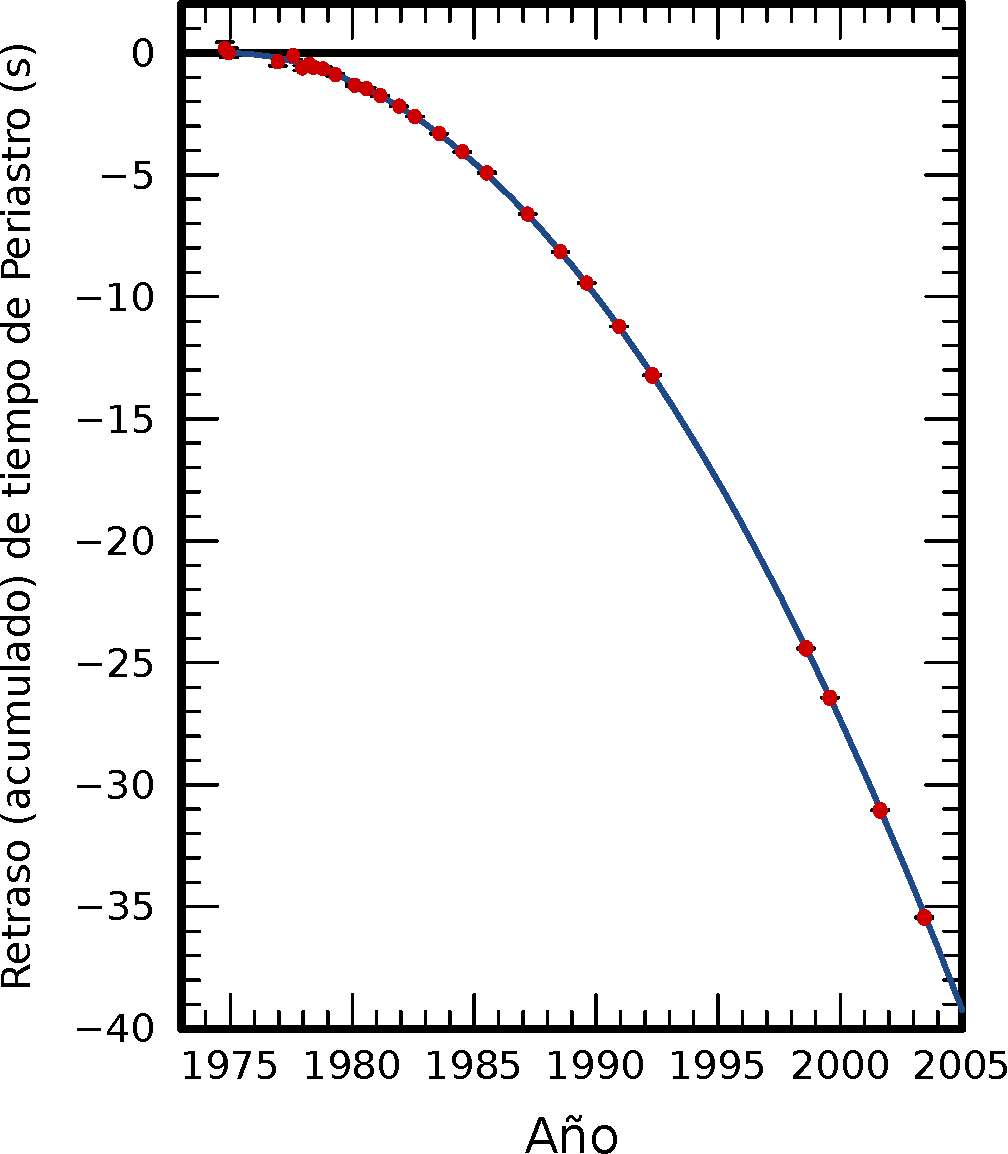
\includegraphics[height=7cm]{fig/fig-HT.pdf}}
\caption{Predicci'on y observaci'on del tiempo en que el pulsar binario de Hulse y Taylor completa cada revolución (tiempo de periastro), respecto al valor newtoniano. Adaptada a partir de \href{http://en.wikipedia.org/wiki/File:PSR_B1913\%2B16_period_shift_graph.svg}{esta} figura original.}
\label{fig:HT}
\end{figure}
\end{center}


\begin{align}
\frac{da}{dt} &= -\frac{64}{5}\frac{G^3\mu M^2}{c^5a^3}\frac{1}{\left(1-e^2\right)^{7/2}}\left(1+\frac{73}{24}e^2+\frac{37}{96}e^4\right) \label{dadt},\\
\frac{de}{dt} &= -\frac{304}{15}\frac{G^3\mu M^2}{c^5a^4}\frac{e}{\left(1-e^2\right)^{5/2}}\left(1+\frac{121}{304}e^2\right). \label{dedt}
\end{align}

En el caso de una 'orbita circular, $e=0$, la ecuaci'on se reduce a
\begin{equation}
\frac{da}{dt} = -\frac{64}{5}\frac{G^3\mu M^2}{c^5a^3},
\end{equation}
cuya soluci'on es...
\begin{equation}
a(t) = \left[a_0^4-\frac{256}{5}\frac{G^3\mu M^2}{c^5}(t-t_0)\right]^{1/4}.
\end{equation}

Dividiendo las ecuaciones \eqref{dadt} \eqref{dedt} para $\dot{a}$ y $\dot{e}$ podemos eliminar el tiempo de estas expresiones y encontrar una ecuaci'on que relaciona directamente $a$ con $e$:
\begin{equation}
\frac{da}{de}=\frac{12}{19}a\frac{1+(73/24)e^2+(37/96)e^4}{e(1-e^2)[1+(121/304)e^2]}.
\end{equation}
La soluci'on de esta ecuaci'on es de la forma
\begin{equation}
a(e)=a_{0}\frac{g(e)}{g(e_{0})},
\end{equation}
con 
\begin{equation}
g(e):= \frac{e^{12/19}}{1-e^2}\left(1+\frac{121}{304} \right)^{870/2299}.
\end{equation}

% \section{Ecuaci'on de movimiento para una part'icula de prueba}
%
% \begin{equation}
% \frac{d^2x^I}{dt^2}=-\Gamma^I_{\ 00}+ \left[\Gamma^0_{\ 00}\delta^I_J-
% 2\Gamma^I_{\ 0J}\right]v^J +\left[2 \Gamma^0_{\ 0J}\delta^I_K -
% \Gamma^I_{\ JK}\right]v^Jv^K + \Gamma^0_{\ JK}v^Iv^Jv^K ,
% \end{equation}
%
% A primer orden en $v$, es decir, en el l'imite no-relativista, podemos
% escribir
%
% \chapter{La apr'oximaci'on post-newtoniana}
%
% The post-Newtonian approximation (see \cite{Wei72,Will93}, also \cite{Sch96})
% applies to systems of slowly moving particles bound together by
% gravitational forces. In such systems the typical values of the Newtonian
% potential $\bar{\phi}\sim\frac{G\bar{M}}{\bar{r}}$
% ($\bar{M}$ and $\bar{r}$ are the typical mass and distance between
% particles) is of the same
% order of magnitude as the typical squared velocities of the particles
% $\bar{v}^2$ (e.g. for a test particle in a circular orbit of radius $r$
% around a central mass $M$ we actually have $v^2=GM/r$).
% The post-Newtonian approximation is based on an expansion of
% the quantities involved in the determination of the trajectories of the
% particles, in powers of the small parameter $v$, taking into account
% that $\mathcal{O}(\phi)\sim \mathcal{O}(v^2)$, and keeping only the first post-Newtonian
% correction in a consistent way. In this section we follow the conventions
% and notation of Weinberg \cite{Wei72} and use $c=1$, and a metric with
% signature $(-,+,+,+)$.
%
% The geodesic equation for a test particle can be written as (see
% \cite{Wei72}, eq. (9.1.2))
% \begin{equation}\label{geo}
% \frac{d^2x^i}{dt^2}=-\Gamma^i_{\ 00}-2\Gamma^i_{\ 0j}v^j -
% \Gamma^i_{\ jk}v^jv^k +\left[\Gamma^0_{\ 00} +2 \Gamma^0_{\ 0j}v^j +
% \Gamma^0_{\ jk}v^jv^k\right]v^i \, es decir,
% \end{equation}
% where we are using coordinates $x^\mu=(t,x^i)$, $i=1,2,3$,
% $v^i:=\frac{dx^i}{dt}$ and $\Gamma^\mu_{\ \nu\lambda}$ are the
% Christoffel symbols corresponding to the metric tensor $g$
% describing the gravitational field of the system.
%
% In the Newtonian approximation, one neglects all velocities and identifies
% $g_{00}\approx -1-2\phi$ so that one recovers the Newtonian law
% \begin{equation}\label{na}
% \frac{d^2x^i}{dt^2}=-\Gamma^i_{\ 00}\approx \frac{1}2\,\delta^{ij}
% \frac{\partial g_{00}}{\partial x^j}\approx -\delta^{ij}
% \frac{\partial \phi}{\partial x^j} .
% \end{equation}
% One then sees that (\ref{na}) contains only terms from (\ref{geo}) up
% to order $v^2/r$. Therefore, in the post-Newtonian approximation, one wants
% to compute (\ref{geo}) up to the next order, which in this case corresponds
% to order $v^4/r$. To carry out this procedure one consider the derivatives
% $\frac{\partial}{\partial x^i}$ and $\frac{\partial}{\partial t}$ as of
% order $1/r$ and $v/r$ respectively.
%
% One can see from (\ref{geo}) that one needs to know the Christoffel
% symbols to the following orders of accuracy: $\Gamma^i_{\ 00}$ to order
% $v^4/r$, $\Gamma^i_{\ 0j}$ to order $v^3/r$, $\Gamma^i_{\ jk}$ to order
% $v^2/r$, $\Gamma^0_{\ 00}$ to order $v^3/r$, $\Gamma^0_{\ 0j}$ to order
% $v^2/r$ and $\Gamma^0_{\ jk}$ to order $v/r$.
% For that, it is enough to compute the metric tensor to the following orders:
% $g_{00}$ to order $v^4$, $g_{0i}$ to order $v^3$ and $g_{ij}$ to order $v^2$.
% In this way, one uses expansions of the form
% \begin{eqnarray}
% g_{00}&=&-1+\stackrel{(2)}g_{00} + \stackrel{(4)}g_{00} + \dots \, es decir,
% \\
% g_{0i}&=&\stackrel{(3)}g_{0i} + \dots \, es decir, \\
% g_{ij}&=&\delta_{ij}+\stackrel{(2)}g_{ij} + \dots \, .
% \end{eqnarray}
%
% With this expansion and a similar one for the matter energy-momentum tensor,
% i.e.
% \begin{eqnarray}
% T^{00}&=&\stackrel{(0)}{T^{00}} + \stackrel{(2)}{T^{00}}+ \dots \, es decir,
% \\
% T^{0i}&=&\stackrel{(1)}{T^{0i}} + \stackrel{(3)}{T^{0i}}+ \dots \, es decir,
% \\
% T^{ij}&=&\stackrel{(2)}{T^{ij}} + \stackrel{(4)}{T^{ij}}+ \dots \, es decir,
% \end{eqnarray}
% one can develop the Einstein eqs.
% \begin{equation}
% R_{\mu\nu}=-8\pi G\left(T_{\mu\nu}-\frac{1}2\, g_{\mu\nu}T^\lambda_{\
% \lambda} \right)\, es decir,
% \end{equation}
% in order to obtain equations for the functions entering in the expansion of
% the metric coefficients. A great simplification is achieved by using
% coordinates satisfying the harmonic coordinate condition
% $g^{\mu\nu}\Gamma^\lambda_{\ \mu\nu}=0$. With this coordinate gauge, the
% Einstein equations reduce to \cite{Wei72}:
% \begin{eqnarray}
% \nabla^2 \stackrel{(2)}g_{00}&=&-8\pi G \stackrel{(0)}{T^{00}} \, es decir, \\
% \nabla^2 \stackrel{(4)}g_{00}&=& \frac{\square \stackrel{(2)}g_{00}}
% {\partial t^2} + \stackrel{(2)}g_{ij}\frac{\square \stackrel{(2)}g_{00}}
% {\partial x^i \partial x^j} - \left(\frac{\partial \stackrel{(2)}g_{00}}
% {\partial x^i}\right) \left(\frac{\partial \stackrel{(2)}g_{00}}
% {\partial x^i}\right) \nonumber \\
% && - 8\pi G\left[\stackrel{(2)}{T^{00}}- 2\stackrel{(2)}g_{00}
% \stackrel{(0)}{T^{00}} + \stackrel{(2)}{T^{ii}}\right] \, es decir, \\
% \nabla^2 \stackrel{(3)}g_{0i}&=&+16\pi G \stackrel{(1)}{T^{0i}} \, es decir,
% \\
% \nabla^2 \stackrel{(2)}g_{ij}&=&-8\pi G \delta_{ij}\stackrel{(0)}{T^{00}} .
% \end{eqnarray}
% The solution of these equations is given by
% \begin{eqnarray}
% \stackrel{(2)}g_{00}&=&-2\phi \, es decir, \\
% \stackrel{(4)}g_{00}&=&-2\phi^2 -2\psi \, es decir, \\
% \stackrel{(3)}g_{0i}&=&\xi_i \, es decir, \\
% \stackrel{(2)}g_{ij}&=&-2\delta_{ij}\phi \, es decir,
% \end{eqnarray}
% where
% \begin{eqnarray}
% \phi&:=&-G\int d^3 x^\prime \frac{\stackrel{(0)}{T^{00}}({\bf x}^\prime,t)}
% {\left|\bf x-x^\prime\right|} ,\\
% \psi&:=&-\int \frac{d^3 x^\prime}{\left|\bf x-x^\prime\right|}\left[
% \frac{1}{4\pi}\, \frac{\square \phi({\bf x}^\prime,t)}{\partial t^2} +
% G \stackrel{(2)}{T^{00}}({\bf x}^\prime,t)+G\stackrel{(2)}{T^{ii}}
% ({\bf x}^\prime,t) \right], \\
% \xi_i&:=&-4G\int d^3 x^\prime \frac{\stackrel{(1)}{T^{0i}}({\bf x}^\prime,t)}
% {\left|\bf x-x^\prime\right|} .
% \end{eqnarray}
%
%
% In summary, in the post-Newtonian approximation the metric tensor is given by
% \begin{eqnarray}
% g_{00}&=&-1 -2\phi -2\phi^2 -2\psi + \mathcal{O}(v^6),\\
% g_{0i}&=&\xi_i + \mathcal{O}(v^5),\\
% g_{ij}&=&\delta_{ij}\left(1-2\phi\right) +\mathcal{O}(v^4)\, .
% \end{eqnarray}
% The geodesic eq. (\ref{geo}) in vector notation takes the form
% (see \cite{Wei72}, eq. (9.2.1)):
% \begin{eqnarray}
% \frac{d\vec{v}}{dt}&=&-\vec{\nabla}\left(\phi +2\phi^2+\psi\right)
% -\frac{\partial\vec{\xi}}{\partial t} + \vec{v}\, \times\left(\vec{\nabla}
% \times \vec{\xi}\right) \nonumber \\
% && + 3\vec{v}\, \frac{\partial\phi}{\partial t}+4\vec{v}
% \left(\vec{v}\cdot\vec{\nabla}\right)\phi -v^2\vec{\nabla}\phi +\mathcal{O}(v^6/r) \, .
% \end{eqnarray}
%
% \section{Static, spherically symmetric pressureless matter distribution}
%
% %For the case of a static, spherically symmetric matter distribution we have
% %$T^{00}=T^{00}(r)$ and $T^{0i}=0$.
%
% We assume a static, spherically symmetric matter distribution described
% by the energy momentum tensor of dust, so that
% \begin{equation}
% T^{\mu\nu}=\rho\, U^\mu U^\nu\, es decir,
% \end{equation}
% with $U^\mu=\left(\frac{dt}{d\tau},0,0,0\right)$ is the 4-velocity of
% the static matter distribution and $\rho=\rho(r)$ is the rest mass density.
% In this case only $T^{00}$ is different from zero and, in particular :
% %(\cite{Wei72}, eqs. (9.3.8)- (9.3.11)):
% \begin{eqnarray}
% \stackrel{(0)}{T^{00}}&=&\rho(r) , \\
% \stackrel{(2)}{T^{00}}&=& -2\phi(r)\, \rho(r) \, . \label{dif}
% \end{eqnarray}
%
% %[Now I have obtained the factor 2, in agreement with Will, table 4.1, with
% %$U=-\phi$ and $\Phi_2=-\psi/2$. See also eq. (39.42a) in \cite\cite{MTW73}
%.Now everything seems to be correct.]
%
% Under these simplifications the metric is given by
% \begin{eqnarray}
% g_{00}&=&-1 -2\phi -2\phi^2 -2\psi + \mathcal{O}(v^6),\\
% g_{0i}&=&0 + \mathcal{O}(v^5),\\
% g_{ij}&=&\delta_{ij}\left(1-2\phi\right) +\mathcal{O}(v^4)\, es decir,
% \end{eqnarray}
% with
% \begin{eqnarray}
% \phi&:=&-G\int d^3 x^\prime \frac{\rho(r^\prime)}
% {\left|\bf x-x^\prime\right|} \, es decir, \\
% \psi&:=&2G\int \frac{d^3 x^\prime}{\left|\bf x-x^\prime\right|} \,
% \phi(r^\prime)\, \rho(r^\prime) \, .
% \end{eqnarray}
%
% The geodesic equation reduces to
% \begin{equation}
% \frac{d\vec{v}}{dt}=-\vec{\nabla}\left(\phi +2\phi^2+\psi\right)
% +4\vec{v}\left(\vec{v}\cdot\vec{\nabla}\right)\phi -v^2\vec{\nabla}\phi
% +\mathcal{O}(v^6/r) \, .
% \end{equation}
%
% For a finite matter distribution the potentials $\phi$ and $\psi$ approach
% to zero at infinity. Therefore, the metric is asymptotically the Minskowski
% metric. One then sees, that at infinity, the coordinates employed become
% inertial coordinates. As a result, the associated reference frame at infinity
% is an inertial frame in which the central matter distribution seems to be at
% rest. This corresponds, to an inertial frame comoving with the central mass
% distribution (the center of the galaxy in our case).
%
% However, for a isolated matter distribution, the metric tensor is given
% asymptotically by
% \begin{eqnarray}
% g_{00}&=&-1 +2\frac{G\stackrel{0}{M}}{r} + 2\frac{G\stackrel2{M}}{r}
% + \mathcal{O}(r^{-2},v^6),\\
% g_{0i}&=&0 + \mathcal{O}(v^5),\\
% g_{ij}&=&\delta_{ij}\left(1+2\frac{G\stackrel{0}{M}}{r}\right)
% +\mathcal{O}(r^{-2},v^4)\, es decir,
% \end{eqnarray}
% where
% \begin{equation}
% \stackrel{0}{M}:=\int d^3 x\, \rho ,
% \qquad \stackrel2{M}:=-2\int d^3 x\, \rho\phi \, .
% \end{equation}
%
% Since it is the ``total gravitating mass" $M:=\stackrel{0}{M}+
% \stackrel2{M}$ the one of practical interest (the one
% obtained by studying the motion of test particles far from the central body),
% it is more convenient to replace the rest mass density $\rho$
% in the above equations by the
% ``gravitational mass density" $\rho_g:=\rho\left( 1-
% 2\phi\right)$,
% so that to first post-newtonian order, we can write
% \begin{eqnarray}
% g_{00}&=&-1 -2\phi_g -2\phi_g^2 + \mathcal{O}(v^6),\\
% g_{0i}&=&0 + \mathcal{O}(v^5),\\
% g_{ij}&=&\delta_{ij}\left(1-2\phi_g\right) +\mathcal{O}(v^4)\, es decir,
% \end{eqnarray}
% where
% \begin{equation}
% \phi_g:=-G\int d^3 x^\prime \frac{\rho_g(r^\prime)}
% {\left|\bf x-x^\prime\right|}=\phi+\psi \, .
% \end{equation}
%
% The geodesic eq. then reads,
% \begin{equation}\label{geopn}
% \frac{d\vec{v}}{dt}=-\vec{\nabla}\left(\phi_g +2\phi_g^2\right)
% +4\vec{v}\left(\vec{v}\cdot\vec{\nabla}\right)\phi_g -v^2\vec{\nabla}
% \phi_g +\mathcal{O}(v^6/r) \, .
% \end{equation}
%
% In newtonian terms, this procedure can be thought as a mass renormalization.
% In this context, the total gravitating mass of the system
% ($M=\stackrel{0}{M}+\stackrel2{M}=\int d^3 x\, \rho_g$,
% defined asymptotically) has a contributions from the ``gravitational
% energy'' of the system. Thus, the problem of
% phenomenologically modelling the density $\rho$ is replaced now by the
% problem of modelling $\rho_g$. Since in the applications, we will always use
% this last form of the geodesic equations, we will omit the subindex in
% $\phi_g$ and $\rho_g$ and denote them simply by $\phi$ and $\rho$.
%
% \section{Energy and Angular momentum}
%
% It is possible to define the post-Newtonian generalizations of the
% {\em conserved} quantities corresponding to energy and momentum
% per unit mass in the Newtonian theory.
%
% We define:
% \begin{eqnarray}
% E&:=&\frac{1}2 v^2 + \phi -3\phi v^2 -\phi^2
% %+\psi
% \, es decir, \\
% \vec{l}&:=&(1-4\phi)\, \vec{r}\times\vec{v} \, .
% \end{eqnarray}
%
% Using the equation of motion \ref{geopn}) one shows that these quantities are
% conserved within our approximation:
% \begin{equation}
% \frac{dE}{dt}=0 +\mathcal{O}(v^7/r), \qquad \frac{d\vec{l}}{dt}=\vec{0} + \mathcal{O}(v^6) \,.
% \end{equation}
%
% In the orbit plane, one can use cylindrical coordinates $(r,\varphi)$
% \footnote{As usual $x=r\cos(\varphi)$, $y=r\sen(\varphi)$} and
% find the equation giving the dependence of the angle $\varphi$ in terms of
% $r$. Using the expressions for the conserved quantities in cylindrical
% coordinates, namely
% \begin{eqnarray}
% E&=&\frac{1}2\left(1-6\phi\right)\left[\left(\frac{dr}{dt}\right)^2 +
% r^2 \left(\frac{d\varphi}{dt}\right)^2\right] + \phi -2\phi^2
% %+\psi
% \, es decir, \\
% l&=&\left(1-4\phi\right)\, r^2 \frac{d\varphi}{dt} \, es decir,
% \end{eqnarray}
% one finds
% \begin{equation}
% \frac{l^2}{r^4}\left(\frac{dr}{d\varphi}\right)^2=2(1-2\phi)E-\frac{l^2}{r^2}
% -2\phi +6\phi^2 %-\psi
% +\mathcal{O}(v^6) \, .
% \end{equation}
% Thus, one obtains
% \begin{equation}\label{fideere}
% \frac{d\varphi}{dr}=\pm \frac{l}{r^2}\left[2(1-2\phi)E-\frac{l^2}{r^2}
% -2\phi +6\phi^2 %-\psi
% \right]^{-1/2} \, .
% \end{equation}
%



